\documentclass{article}

\usepackage{color}
\usepackage{graphicx}
\usepackage{amsmath}
\usepackage{float}
 \usepackage{amssymb}
 \usepackage[top=1in, bottom=1in, left=1.25in, right=1.25in]{geometry}
 \usepackage{multirow}
 \usepackage{array}
 \newcommand{\tabincell}[2]{\begin{tabular}
{@{}#1@{}}#2\end{tabular}}

\usepackage{subfig}

\begin{document}

\vspace*{0.25cm}

\hrulefill

\thispagestyle{empty}

\begin{center}
\begin{large}
\sc{SE 276C/MAE 232C: Nolinear and Advanced Finite Elements Method }
\end{large}

\hrulefill

\vspace*{5cm}
\begin{Large}
\sc{
	{Final Project Report, Option 2}}
\end{Large}

	\vspace{7em}
	{Name: Ru Xiang}\\
	\vspace{1.5em}
	{Date: June 12th, 2019}


\end{center}


\vfill


\hfill

\newpage



\section{Problem Statement}

	In this problem, we have a cantilever beam of length $L = 50 in$, height $D = 10 in$, subjected to a shear load $P = 250 lb$ at the end. The beam is made of a hyperelastic material described by Saint Venant-Kirchhoff model.
	


\vspace*{0.5em}
 \begin{figure}[H]
	\centering
	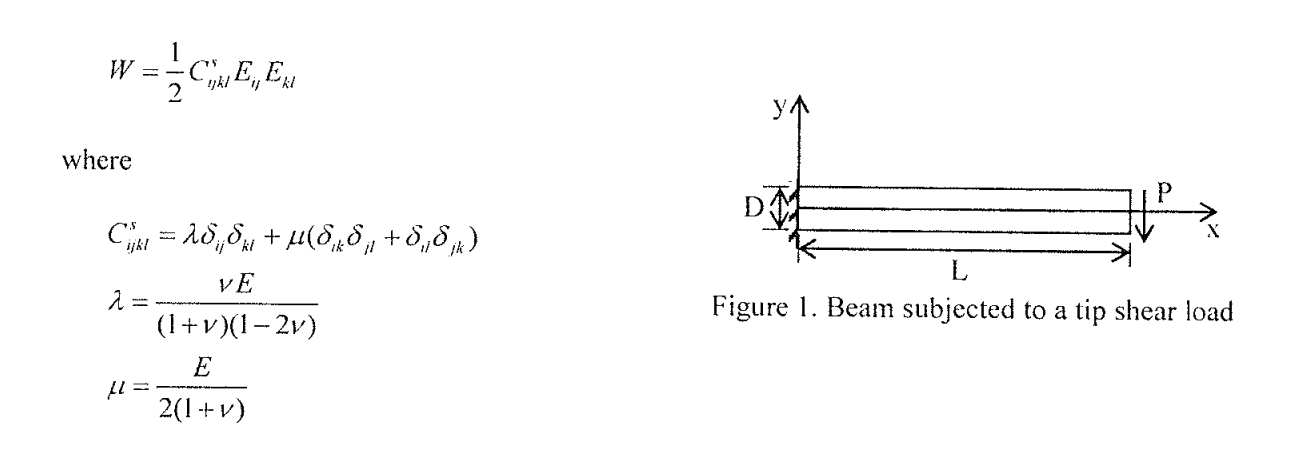
\includegraphics[scale=0.6]{problem.png}
	\caption{2D plane-strain cantilever beam problem.}
\end{figure}

\vspace*{1.5em}
  To solve this problem, we used the following finite element formulations:
  
 \begin{itemize}
 \item 2D plane-strain model, 4-node quadrilateral (Q4) elements.
 \item Saint Venant-Kirchhoff strain engergy density function.
 \item Total Lagrangian Formulation.
 \item Three integration methods: Full Integration \textbf{(FI)}, Reduced Integration \textbf{(RI)} and Selective Reduced Integration \textbf{(SRI)}.
 \end{itemize}

\vspace*{1.5em}


\section{Numerical Formulation and Computational Procedures}

 \begin{figure}[H]
	\centering
	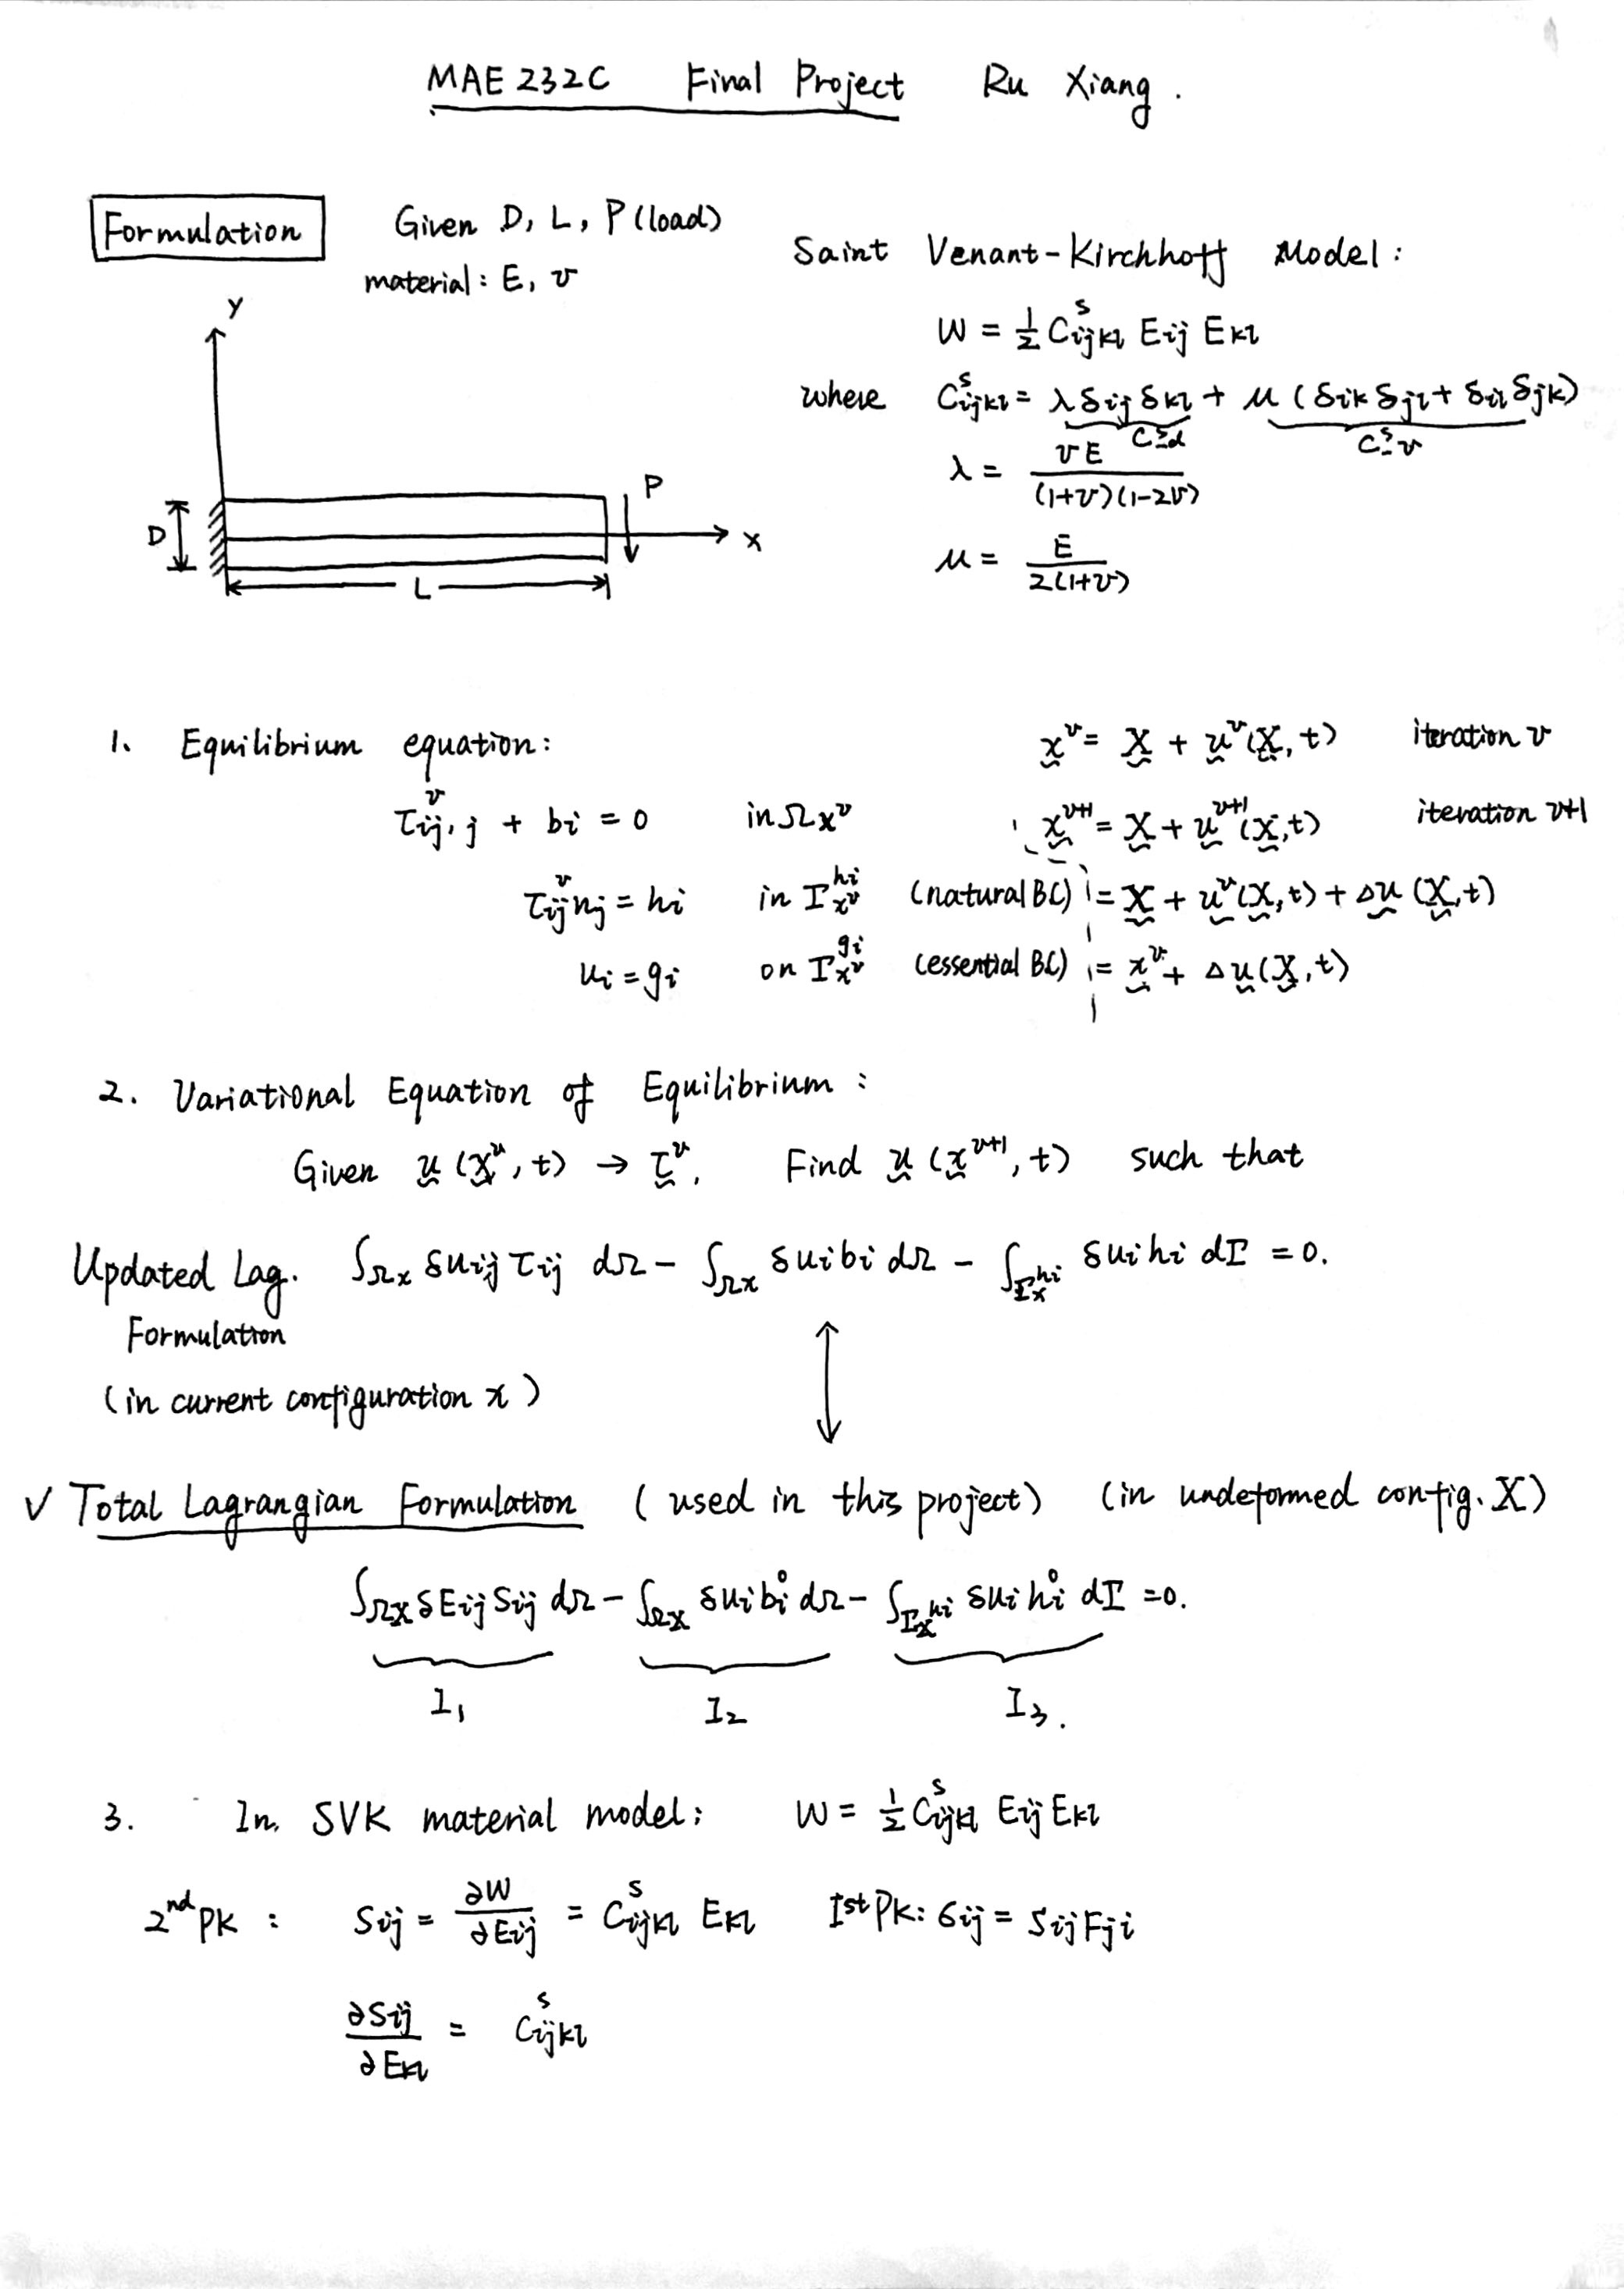
\includegraphics[scale=0.2]{MAE232C_FINAL_PROJECT_latex/formulation_1.jpg}
\end{figure}


\begin{figure}[H]
	\centering
	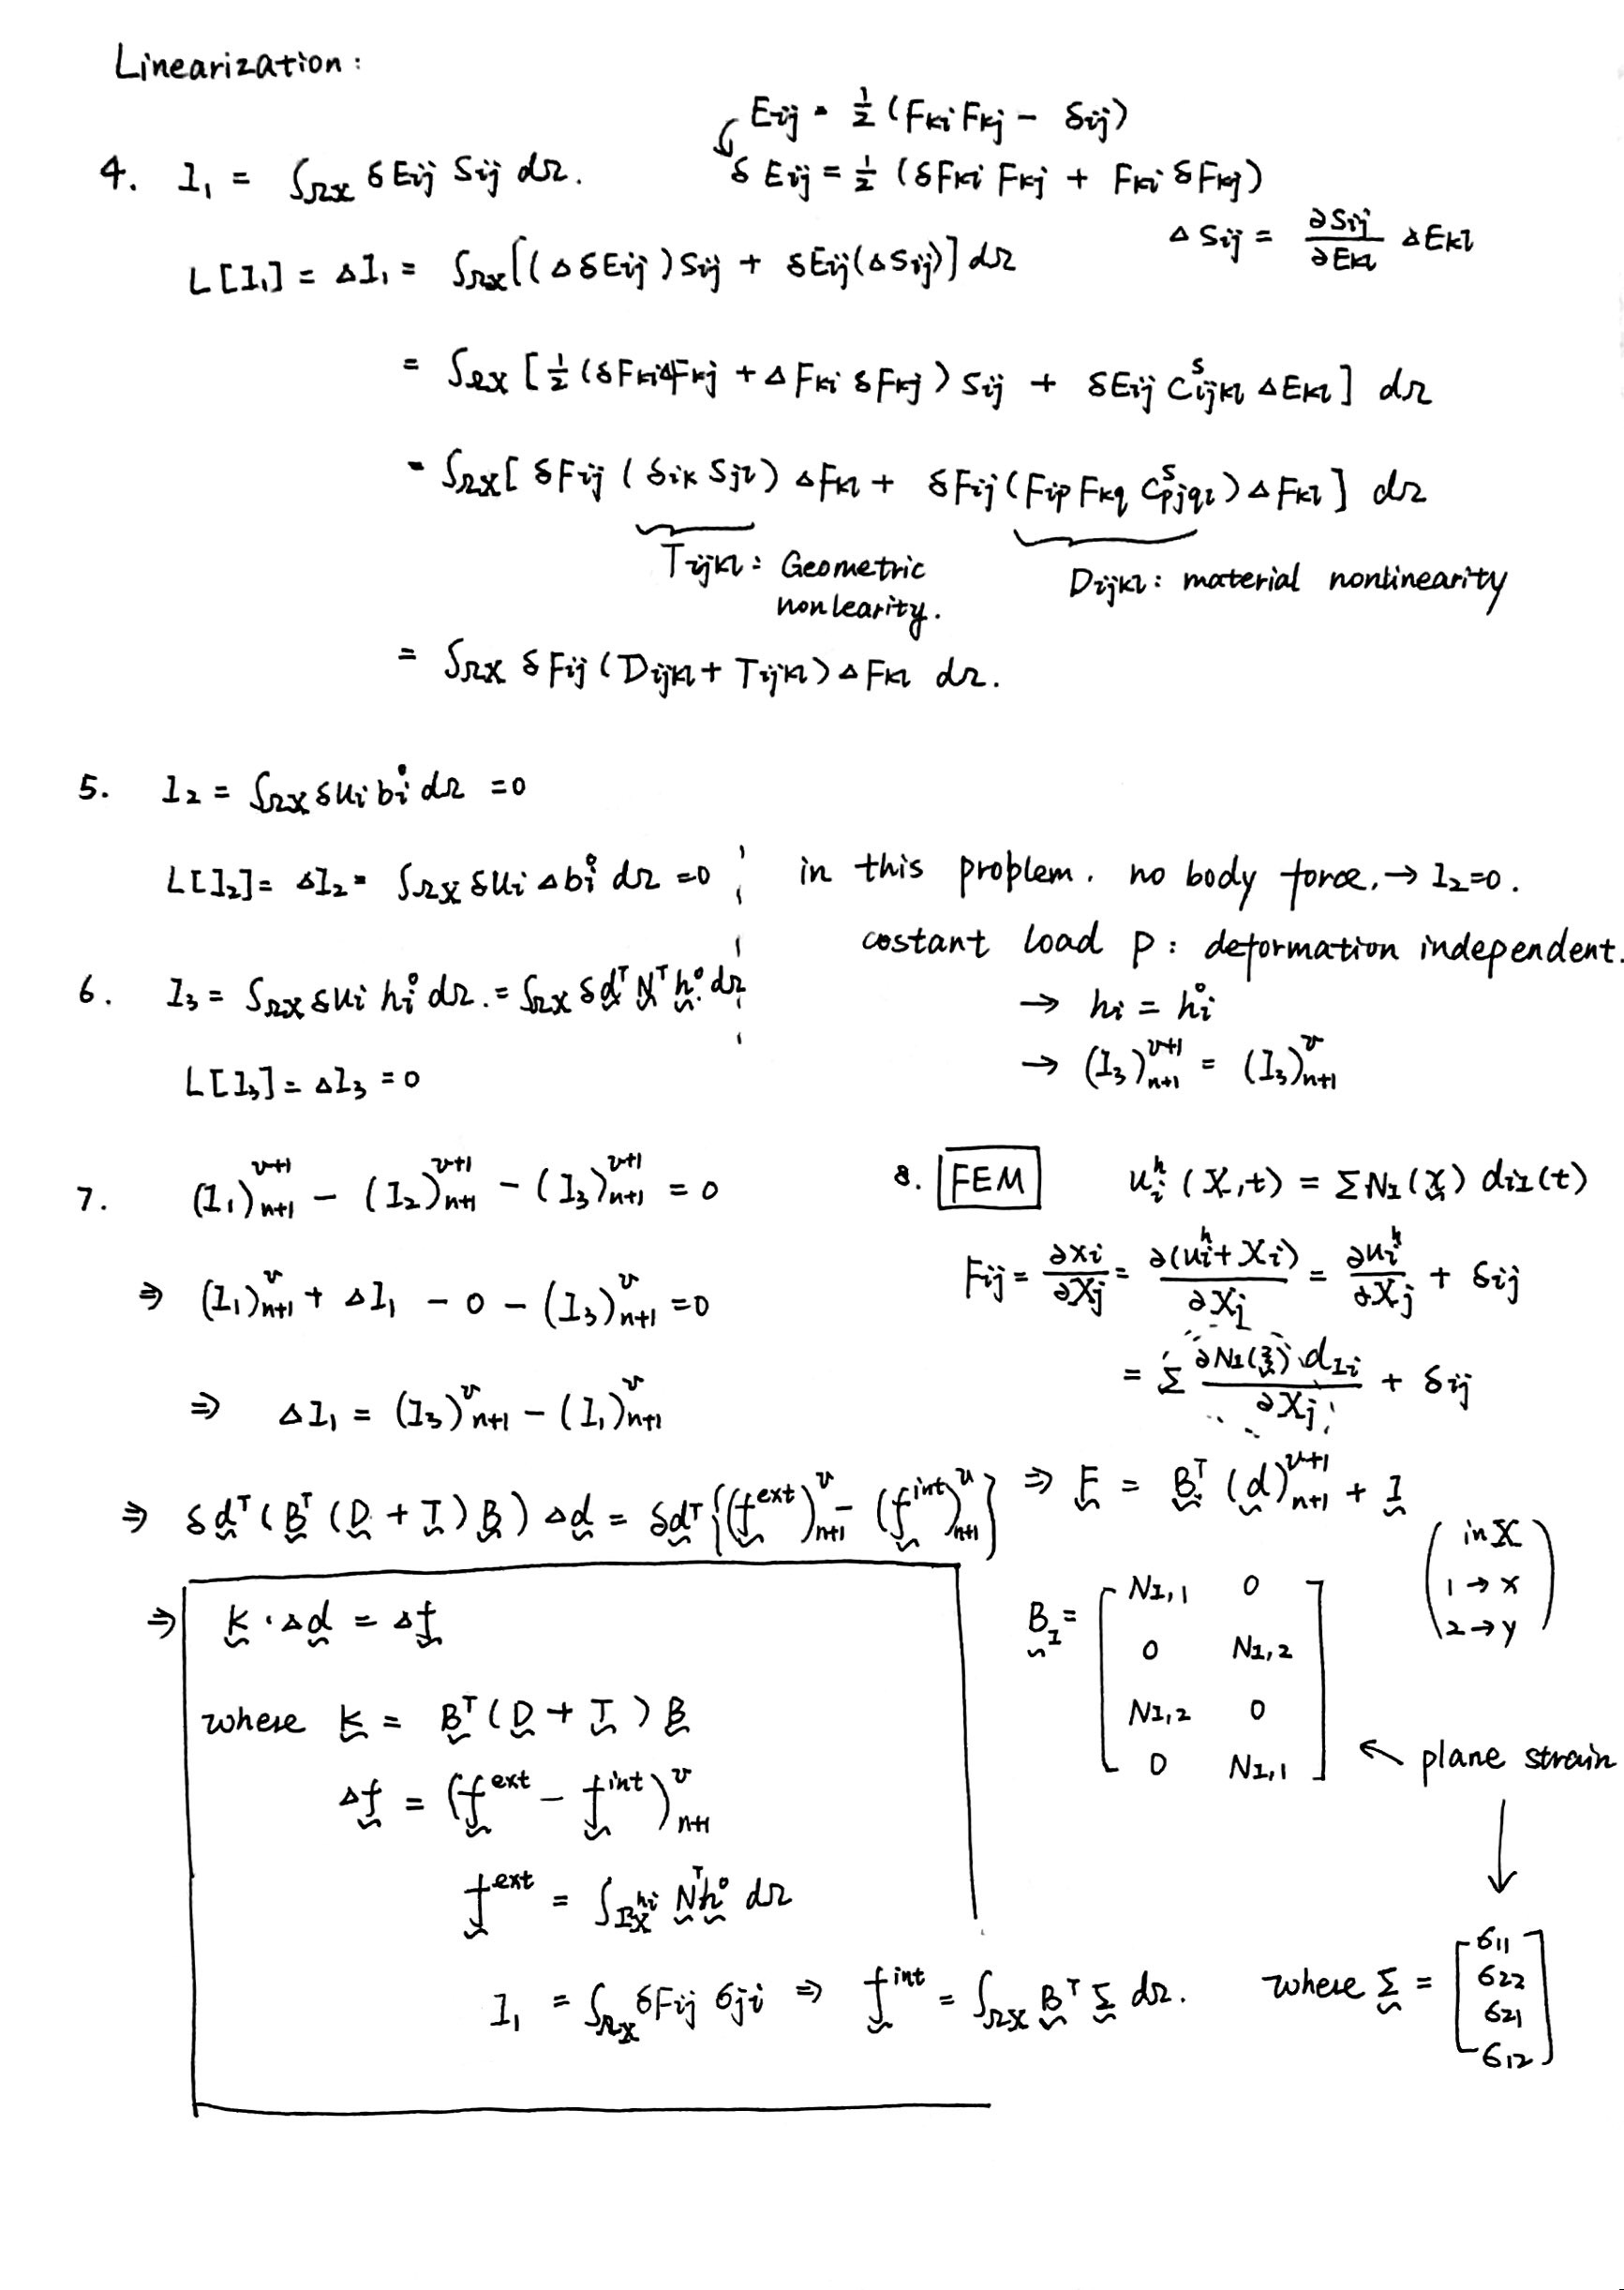
\includegraphics[scale=0.23]{MAE232C_FINAL_PROJECT_latex/formulation_2.jpg}
\end{figure}


\begin{figure}[H]
	\centering
	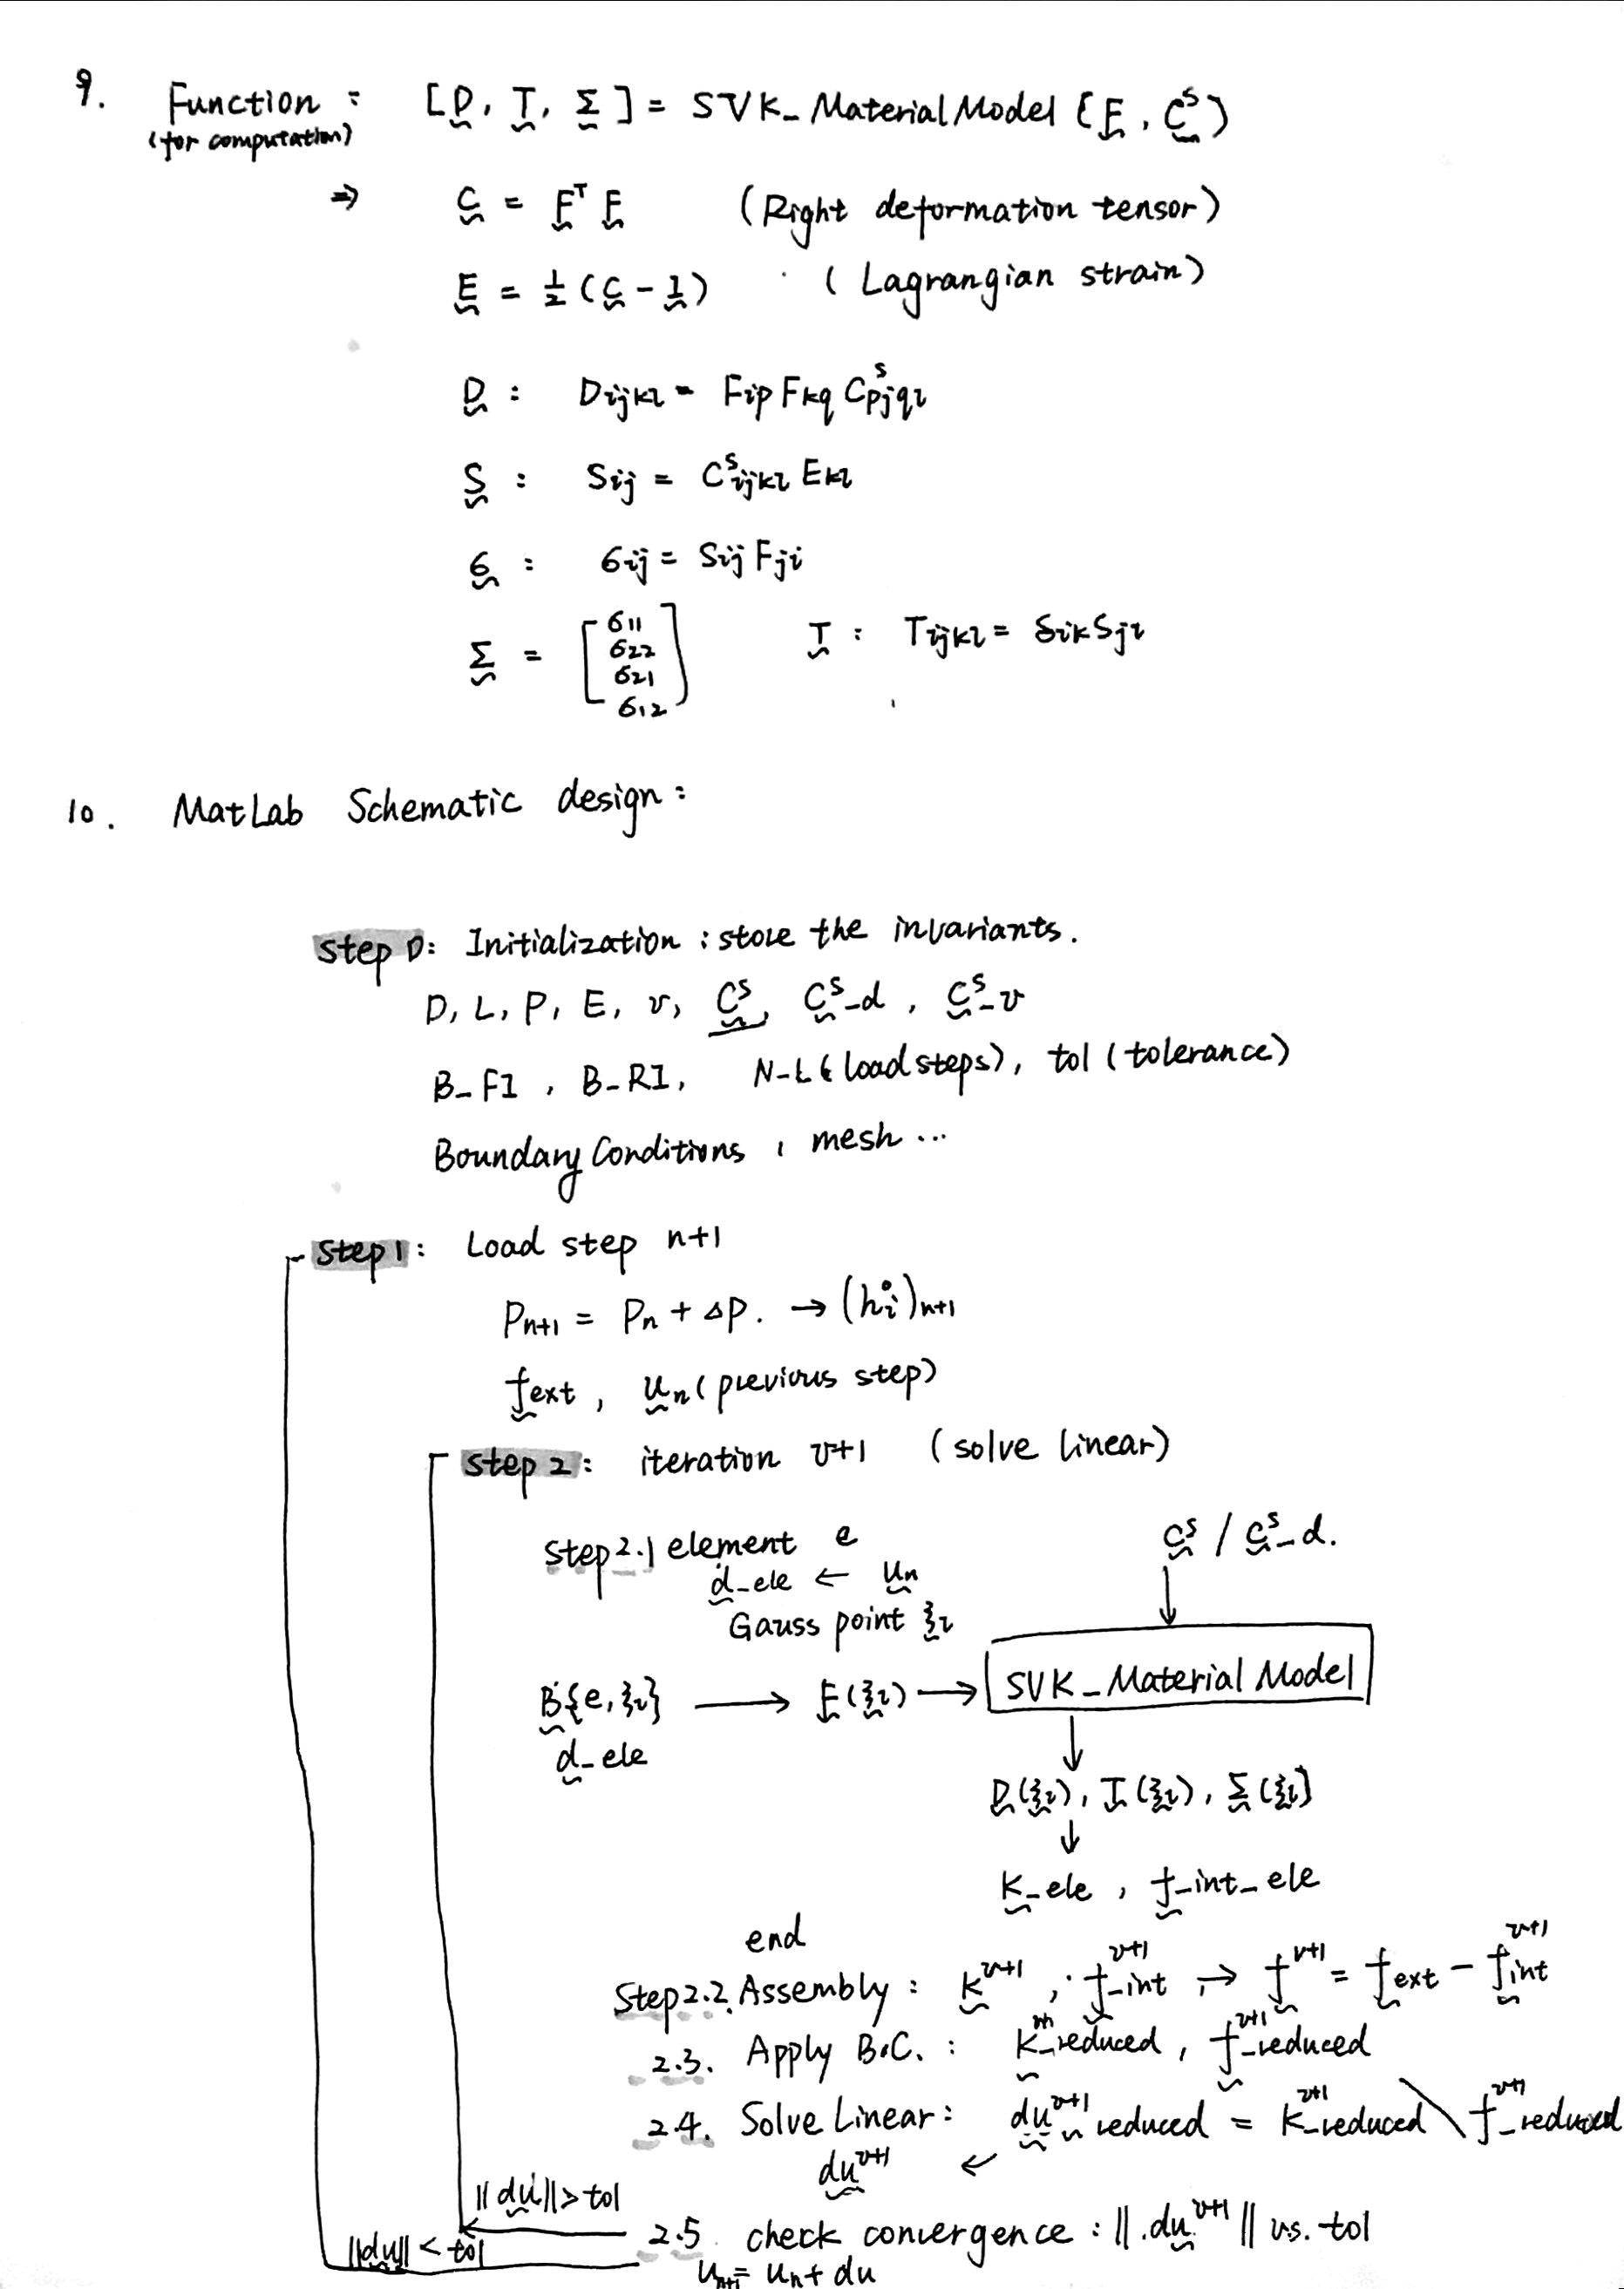
\includegraphics[scale=0.23]{MAE232C_FINAL_PROJECT_latex/formulation_3.jpg}
\end{figure}

\vspace*{1.5em}


\section{Numerical Solutions}
\vspace*{0.5em}
For mesh options of 2x20, 4x40, 8x80, we obtained the numerical results by FI, RI, SRI respectively. All the numerical results were got with settings, load steps = 5 and tolerance for convergence = $10^{-4}$.

\vspace*{0.5em}
\subsection{Load(P) - deflection($u_y$) response at the centroid of the load end}
\vspace*{0.5em}


\begin{figure}[H]
    \centering
    \subfloat[Mesh = 2x20]{{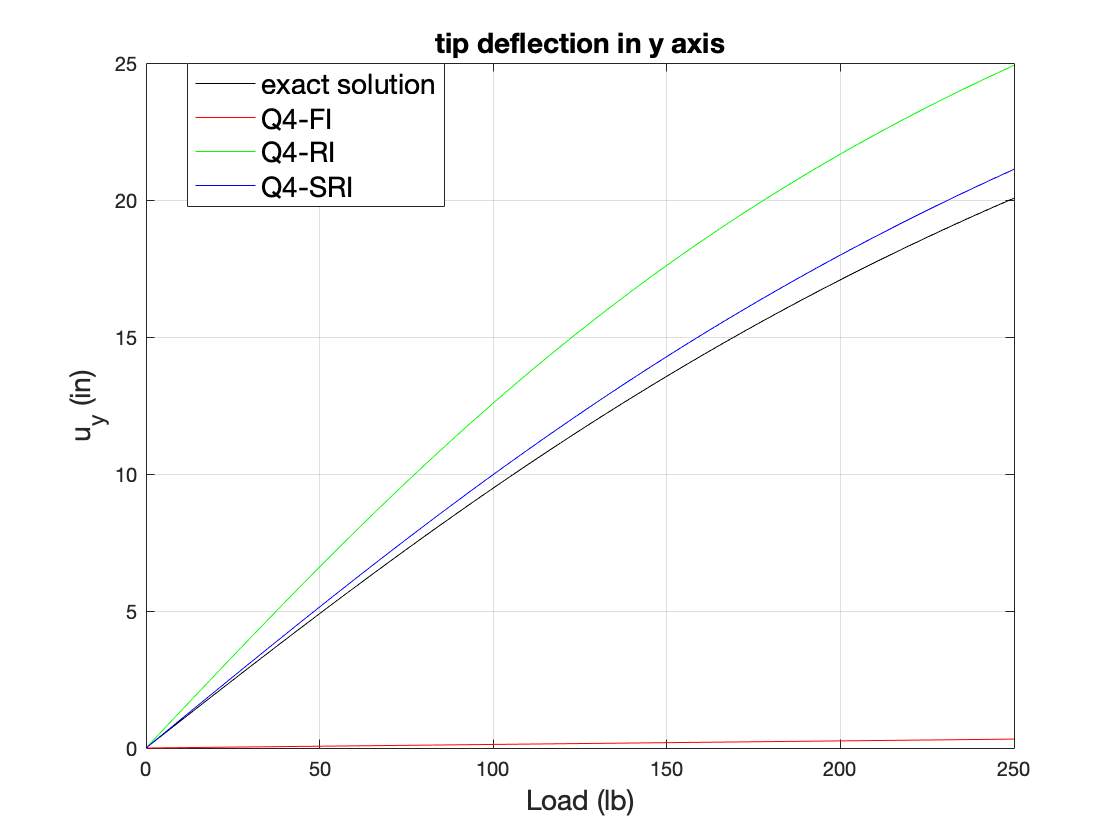
\includegraphics[width=7.1cm]{MAE232C_FINAL_PROJECT_latex/tip_1.png}}}
    \qquad
    \subfloat[Mesh = 4x40]{{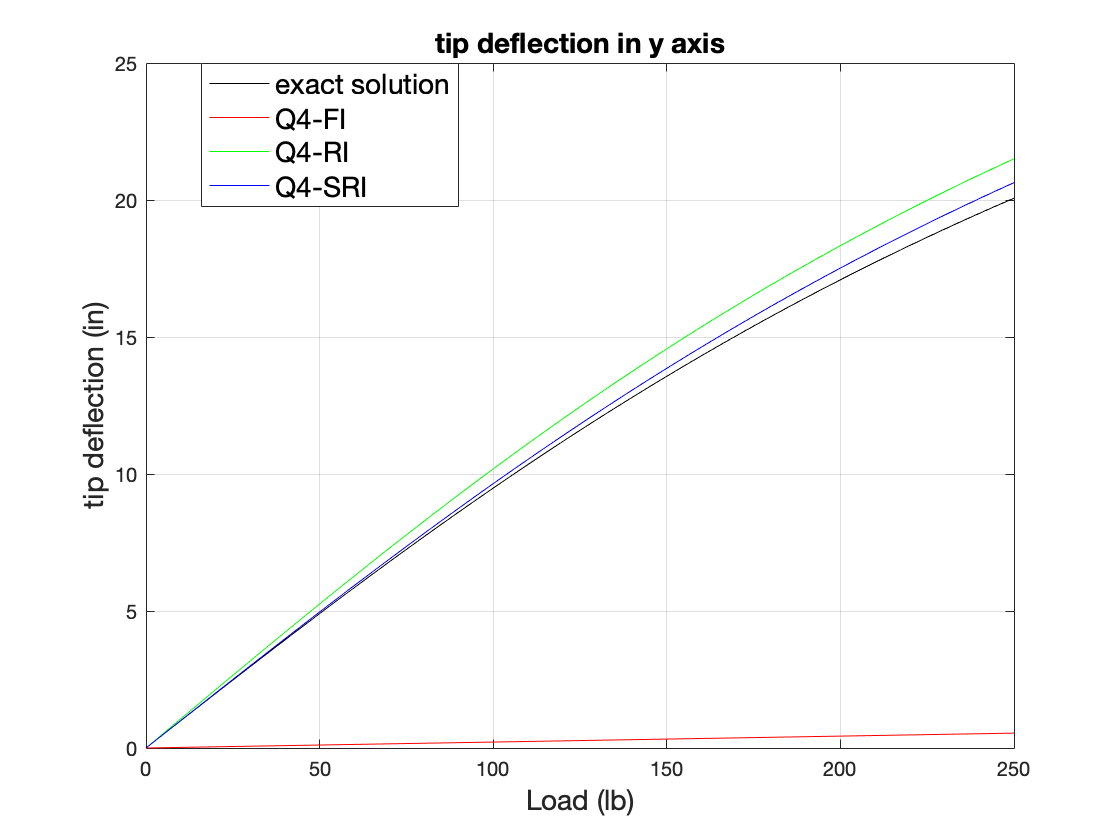
\includegraphics[width=7.1cm]{MAE232C_FINAL_PROJECT_latex/tip_2.png} }}
    \qquad
    \subfloat[Mesh = 8x80]{{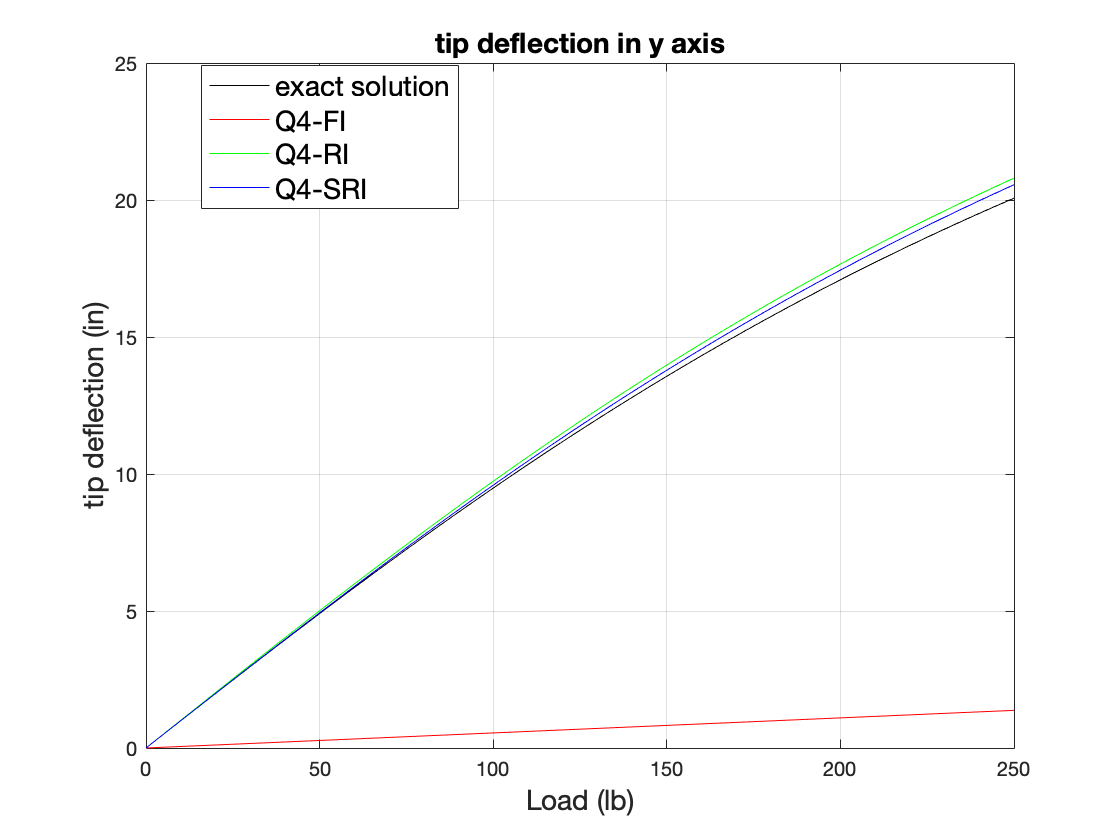
\includegraphics[width=7.1cm]{MAE232C_FINAL_PROJECT_latex/tip_3.png} }}
    \caption{Numerical results of tip deflection with different mesh refinements}
\end{figure}

From the figures above, we can observe that the solutions by FI 'locks' in all the three mesh refinements. However, the results by RI and SRI are very close to the reference solution in (c) mesh = 8x80. And the results by SRI have less error than the results by RI.

\vspace*{0.5em}
\subsection{Displacement solution $u_y$ along $y = 0$ at $P = 250 lb$}
\vspace*{0.5em}

\begin{figure}[H]
    \centering
    \subfloat[Mesh = 2x20]{{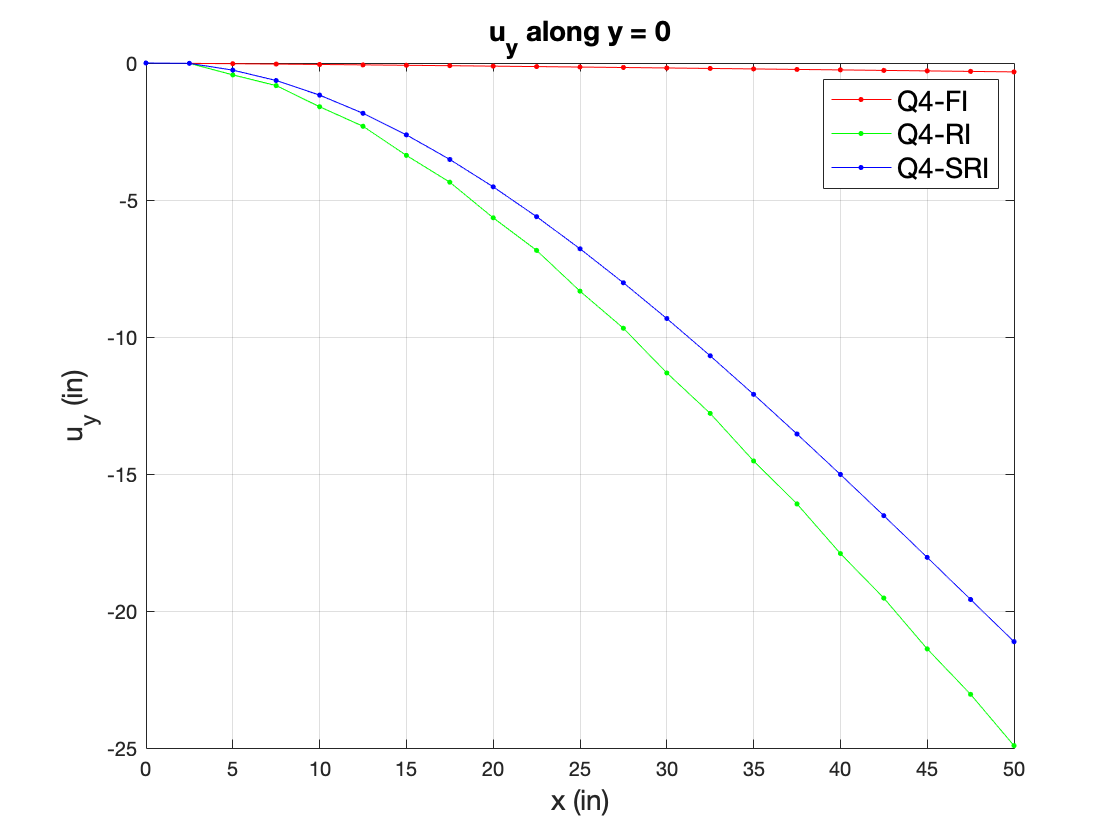
\includegraphics[width=7.1cm]{MAE232C_FINAL_PROJECT_latex/u_0_y_1.png}}}
    \qquad
    \subfloat[Mesh = 4x40]{{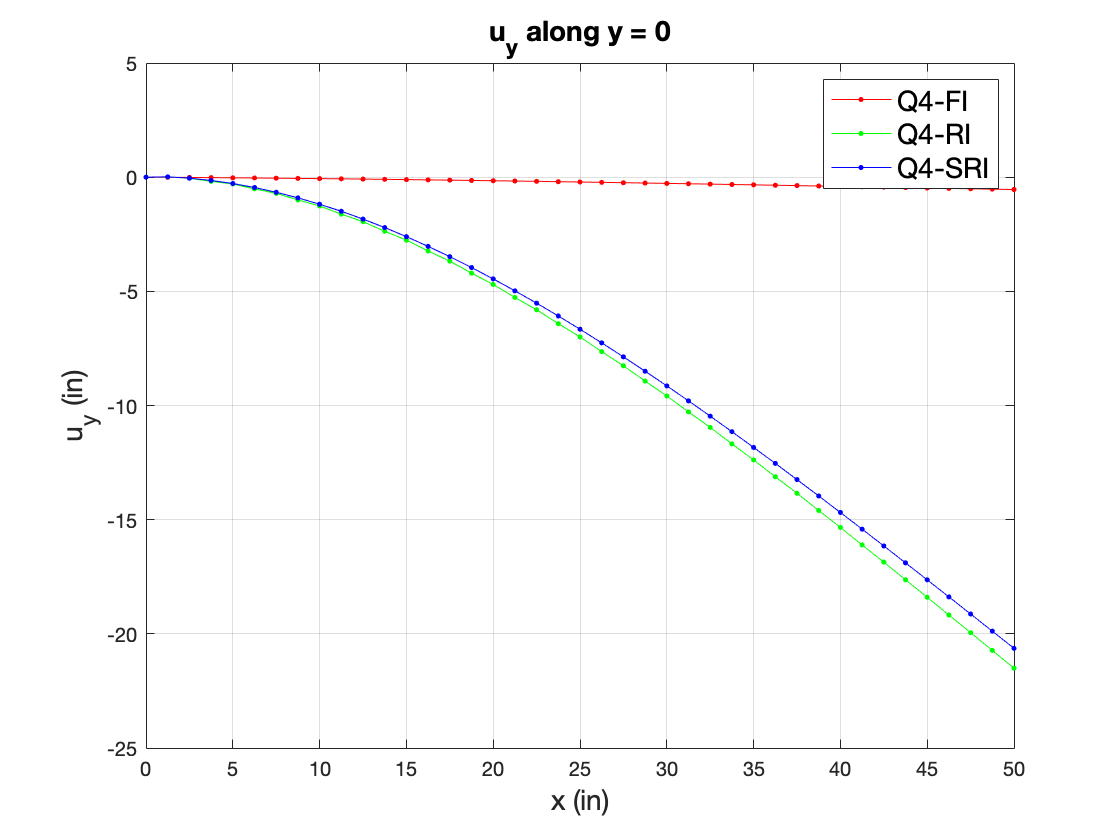
\includegraphics[width=7.1cm]{MAE232C_FINAL_PROJECT_latex/u_0_y_2.png} }}
    \qquad
    \subfloat[Mesh = 8x80]{{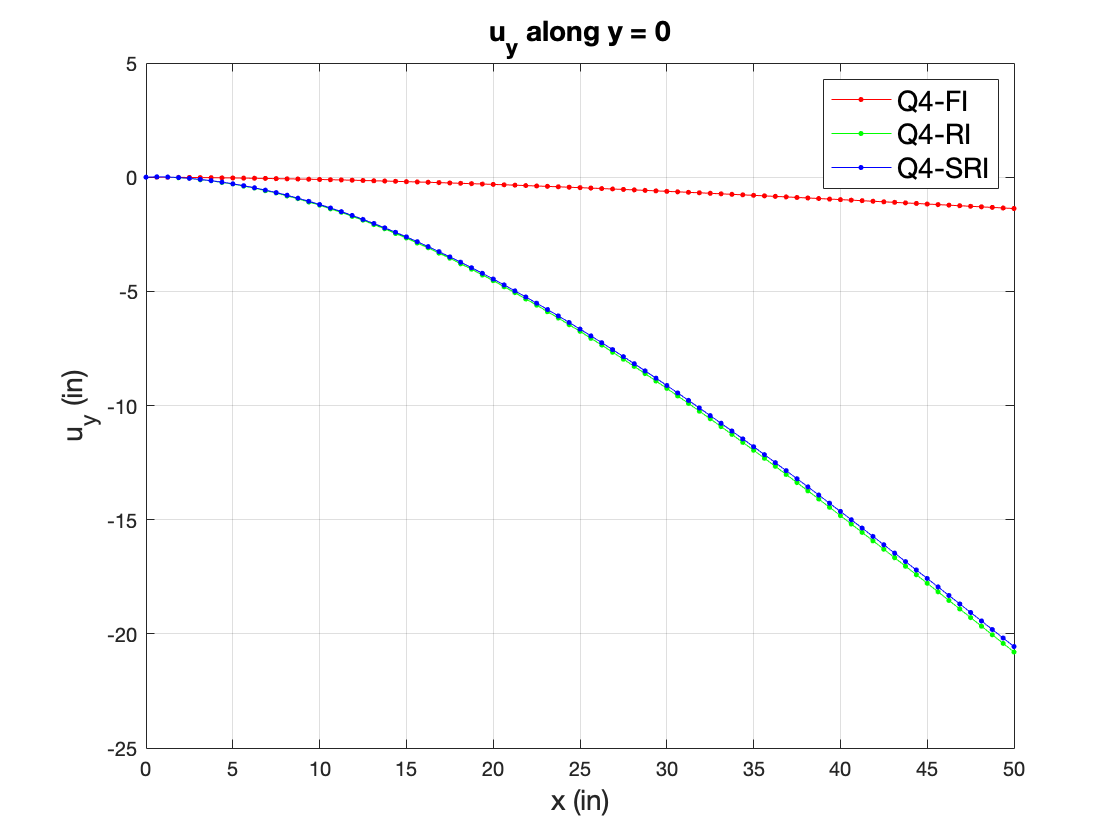
\includegraphics[width=7.1cm]{MAE232C_FINAL_PROJECT_latex/u_0_y_3.png} }}
    \caption{Numerical results of $u_y$ along $y = 0$ with different mesh refinements}
\end{figure}

From the figure above, we can see the results by RI approaches SRI as we refined the mesh, while the results by FI still locks. Then we can implement that we should use refined mesh when using RI in order to get accurate results.


\vspace*{0.5em}
\subsection{Stress solutions along $x = L/2$ at $P = 250 lb$.}
\vspace*{0.5em}

\begin{figure}[H]
    \centering
    \subfloat[Mesh = 2x20]{{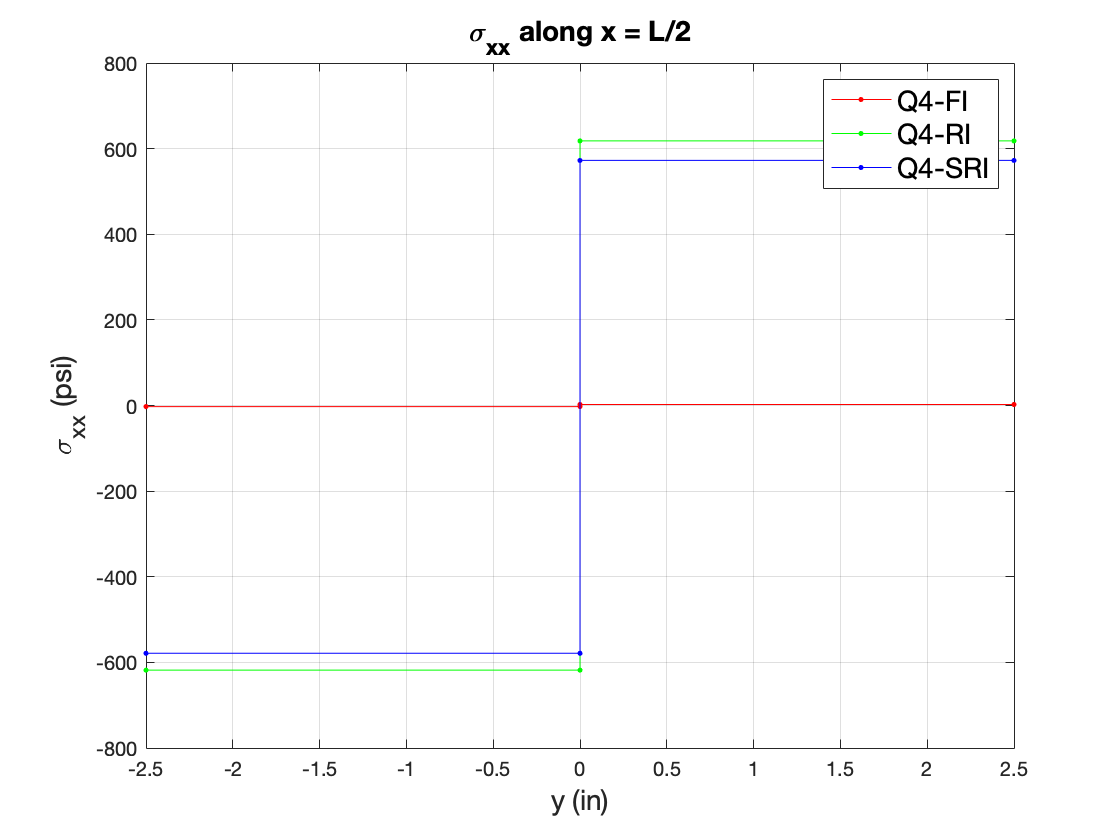
\includegraphics[width=7.1cm]{MAE232C_FINAL_PROJECT_latex/stress_xx_1.png}}}
    \qquad
    \subfloat[Mesh = 4x40]{{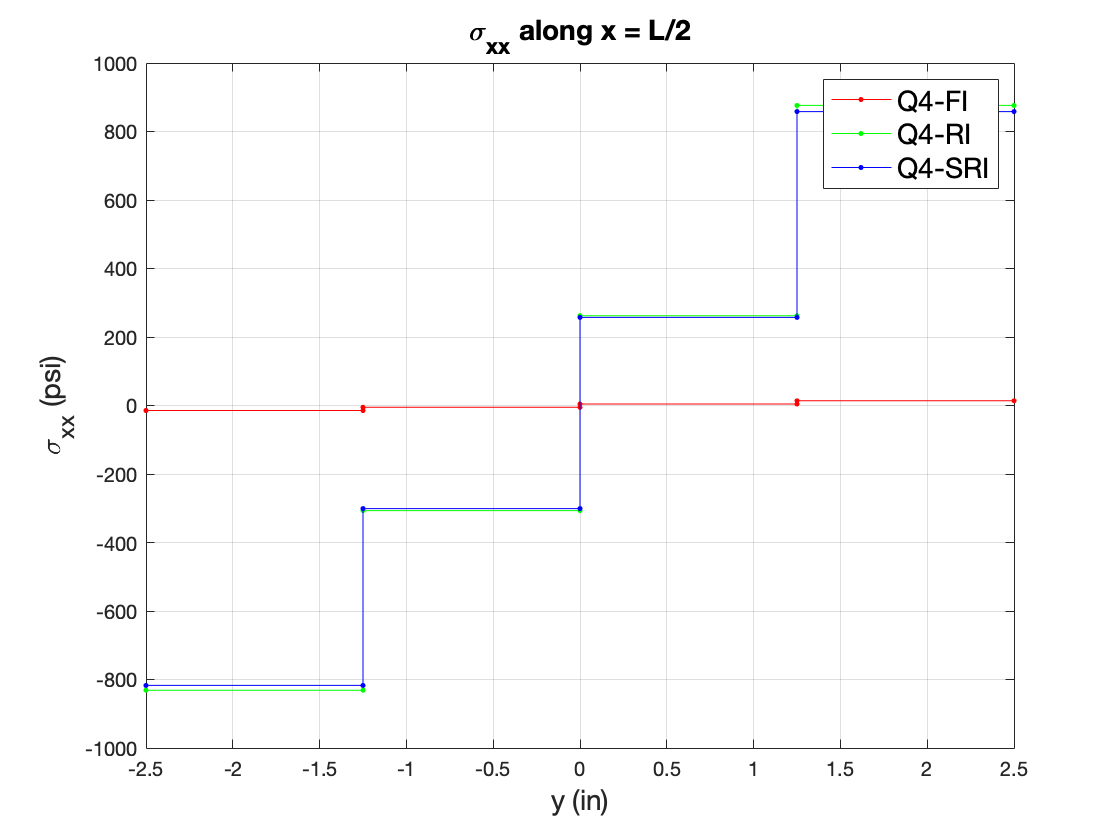
\includegraphics[width=7.1cm]{MAE232C_FINAL_PROJECT_latex/stress_xx_2.png} }}
    \qquad
    \subfloat[Mesh = 8x80]{{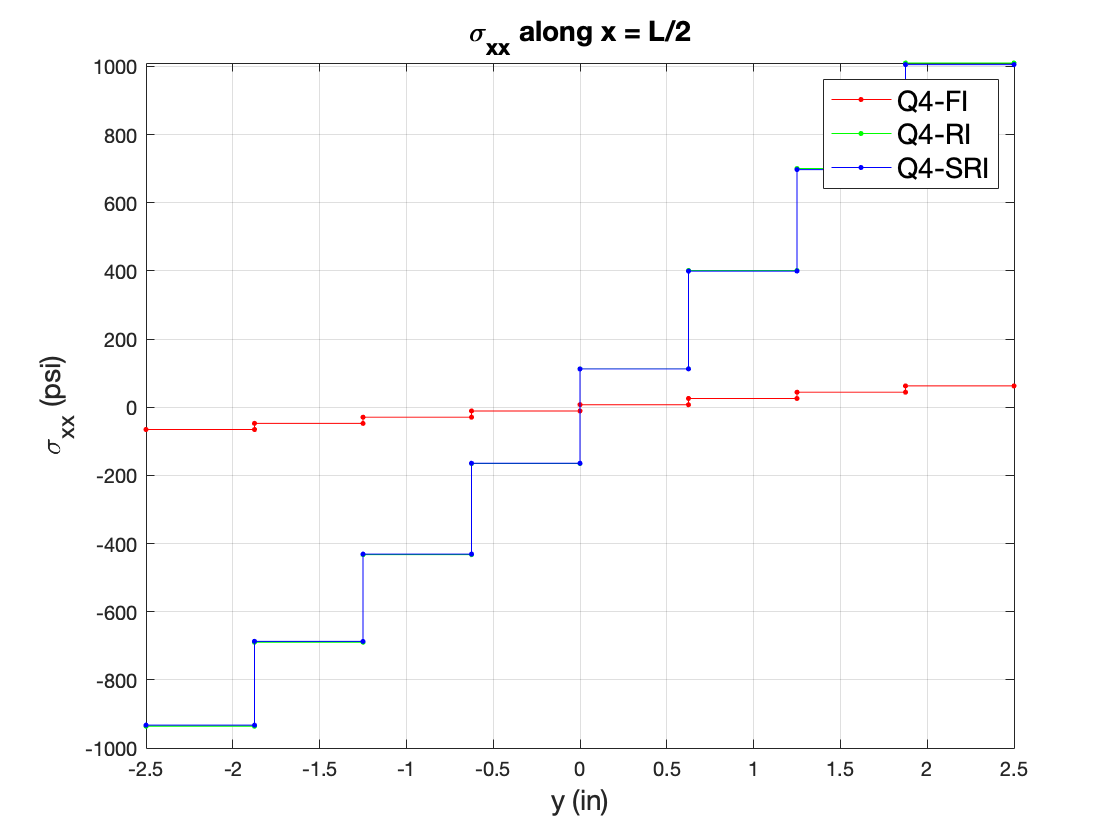
\includegraphics[width=7.1cm]{MAE232C_FINAL_PROJECT_latex/stress_xx_3.png} }}
    \caption{Numerical results of $\sigma_{xx}$ along $x = L/2$ at $P = 250 lb$ with different mesh refinements}
\end{figure}

\begin{figure}[H]
    \centering
    \subfloat[Mesh = 2x20]{{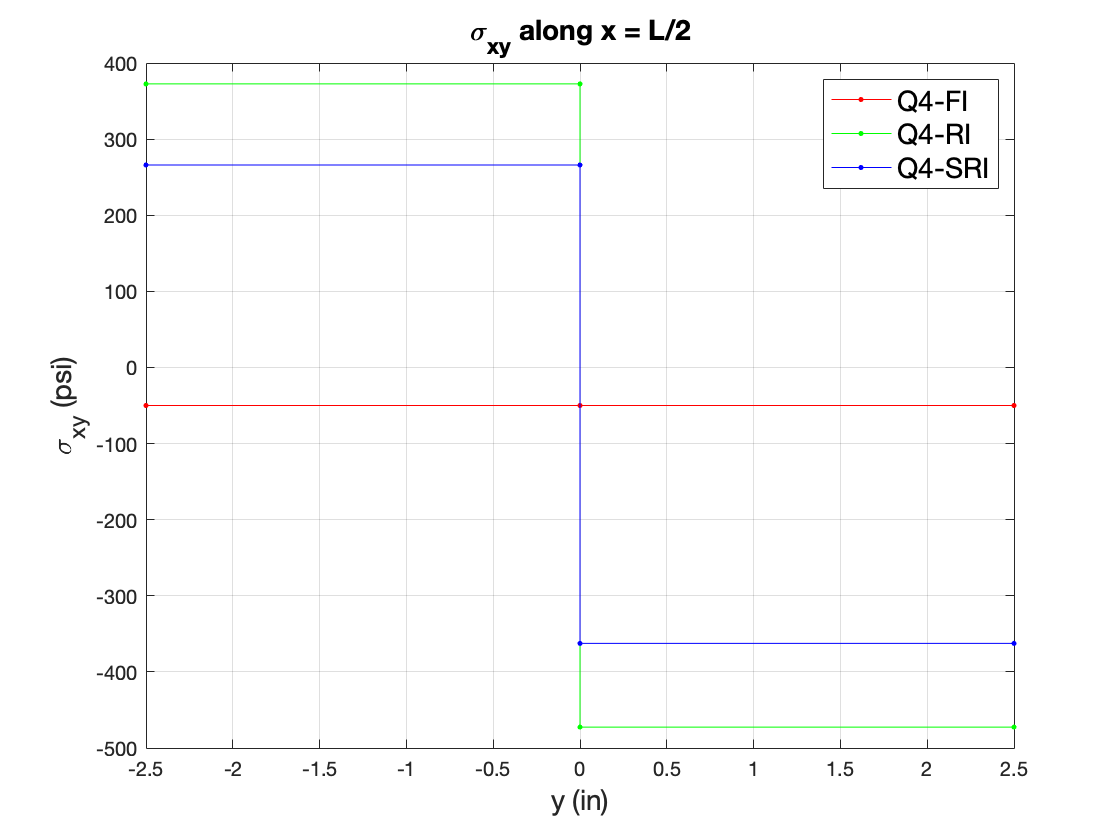
\includegraphics[width=7.1cm]{MAE232C_FINAL_PROJECT_latex/stress_xy_1.png}}}
    \qquad
    \subfloat[Mesh = 4x40]{{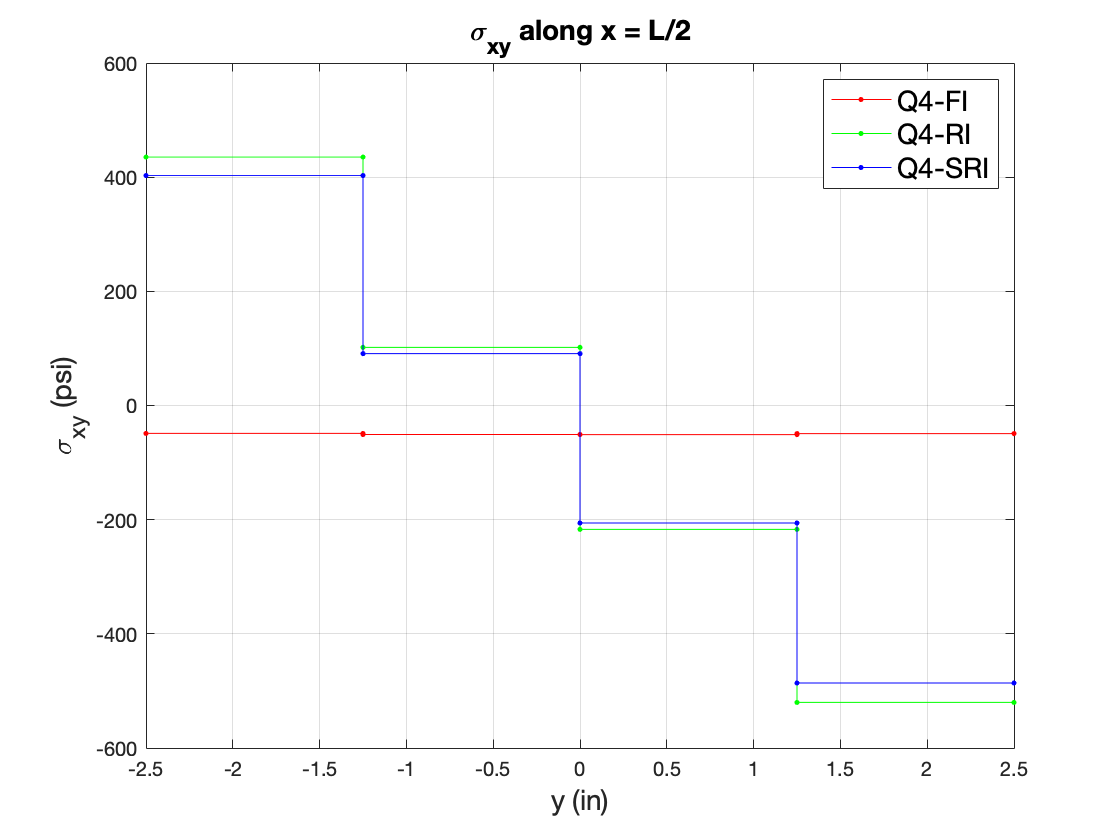
\includegraphics[width=7.1cm]{MAE232C_FINAL_PROJECT_latex/stress_xy_2.png} }}
    \qquad
    \subfloat[Mesh = 8x80]{{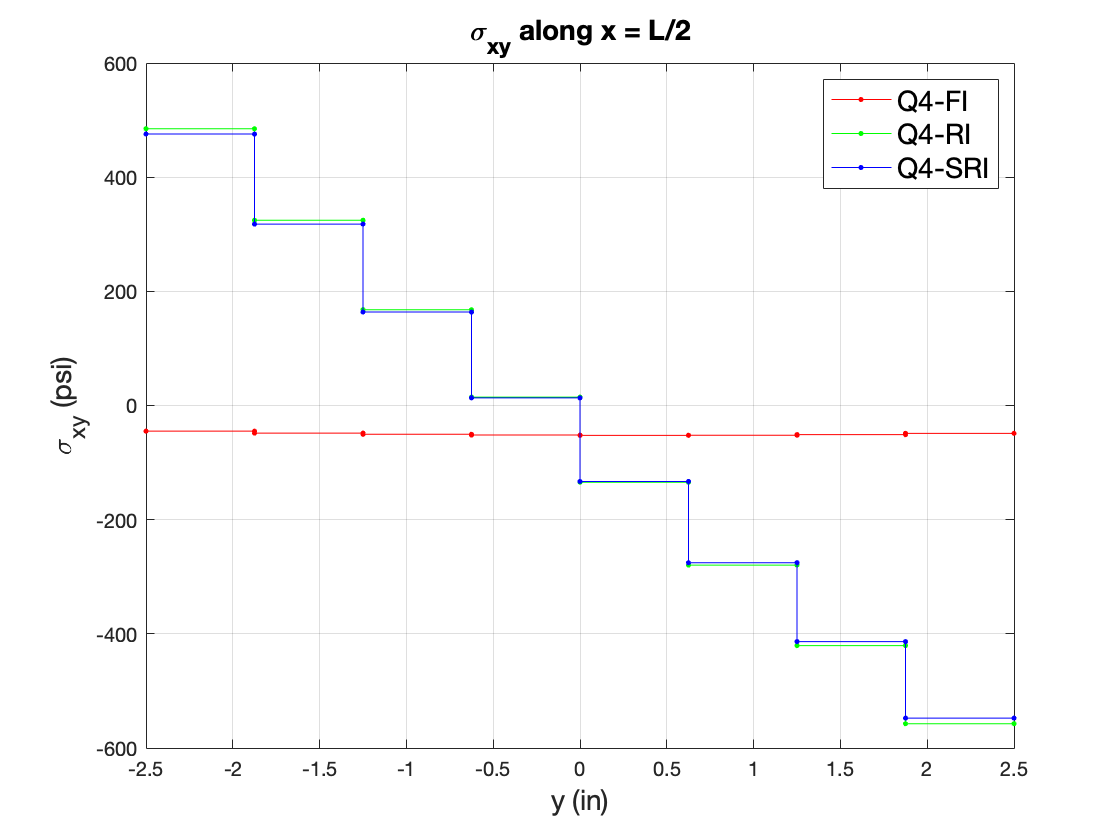
\includegraphics[width=7.1cm]{MAE232C_FINAL_PROJECT_latex/stress_xy_3.png} }}
    \caption{Numerical results of $\sigma_{xy}$ along $x = L/2$ at $P = 250 lb$ with different mesh refinements}
\end{figure}

From the results of $\sigma_{xx}$ and $\sigma_{xy}$ along $x = L/2$ at $P = 250 lb$, we can also observe the 'locking' of FI. And the results of SRI and RI are getting more and more identical to each other when we refined the mesh. And it also meets the mechanical expectation that the stresses increase from $y = 0$ to the upper and lower surfaces.


\section{Discussion}
\subsection{Analysis of the Integration Methods}

\vspace*{0.5em}

The figure below shows the shape of the beam after deformation with different integration methods by 2x20 meshing.

From the numerical results in Section-3, we can observed incompressible locking when using full integration. In Fig.6-a below, it is more obvious that the beam becomes so stiff that it 'locks' even under large load. Then we introduce RI to resolve locking, which only uses one point integration per element. In Fig.6-b, we can see the beam no longer locks. However, there occurs another problem, the Hourglass modes, shown in Fig.6-d: an enlarged part of Fig.6-b. Here we can find the elements have 'zigzags' on element boundary, which are the so-called 'Hourglass modes'. Finally, we used SRI to stabilize the hourglass instability. As we can observe in Fig.6-c, the mesh in the beam becomes smooth and the hourglass modes disappear.

\begin{figure}[H]
    \centering
    \subfloat[Q4-FI]{{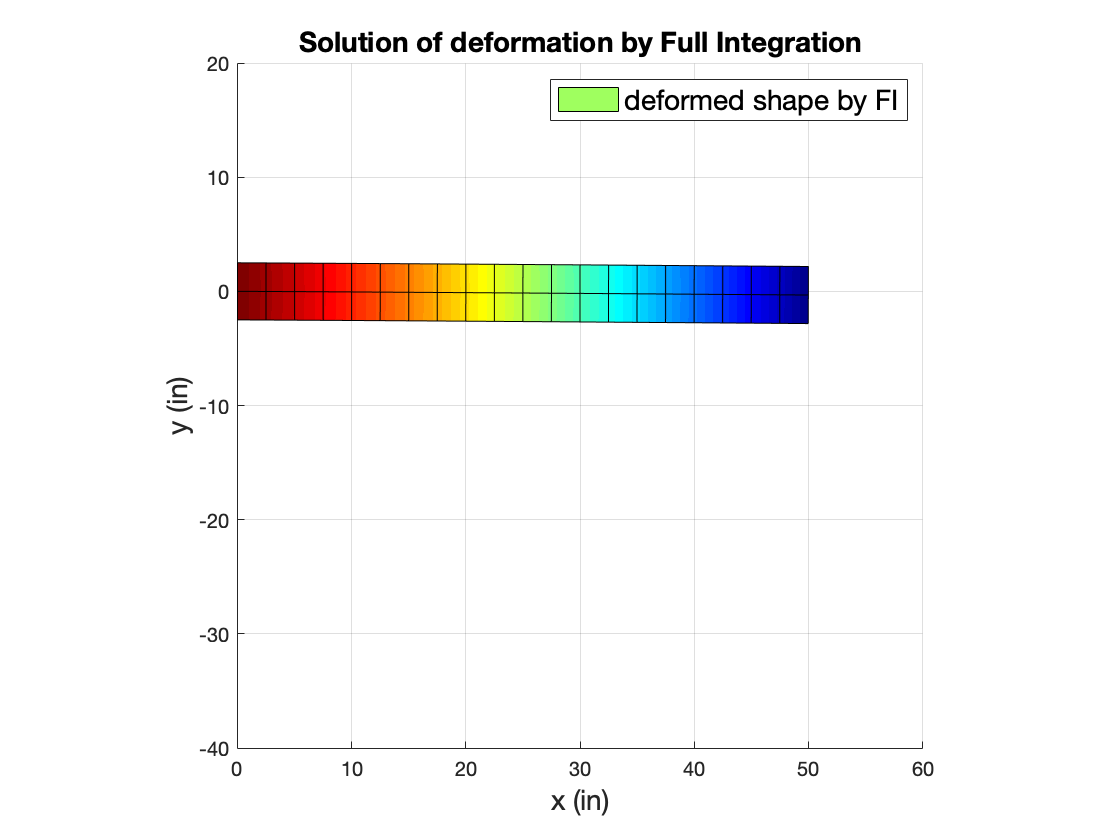
\includegraphics[width=7.1cm]{MAE232C_FINAL_PROJECT_latex/FI_1.png}}}
    \qquad
    \subfloat[Q4-RI]{{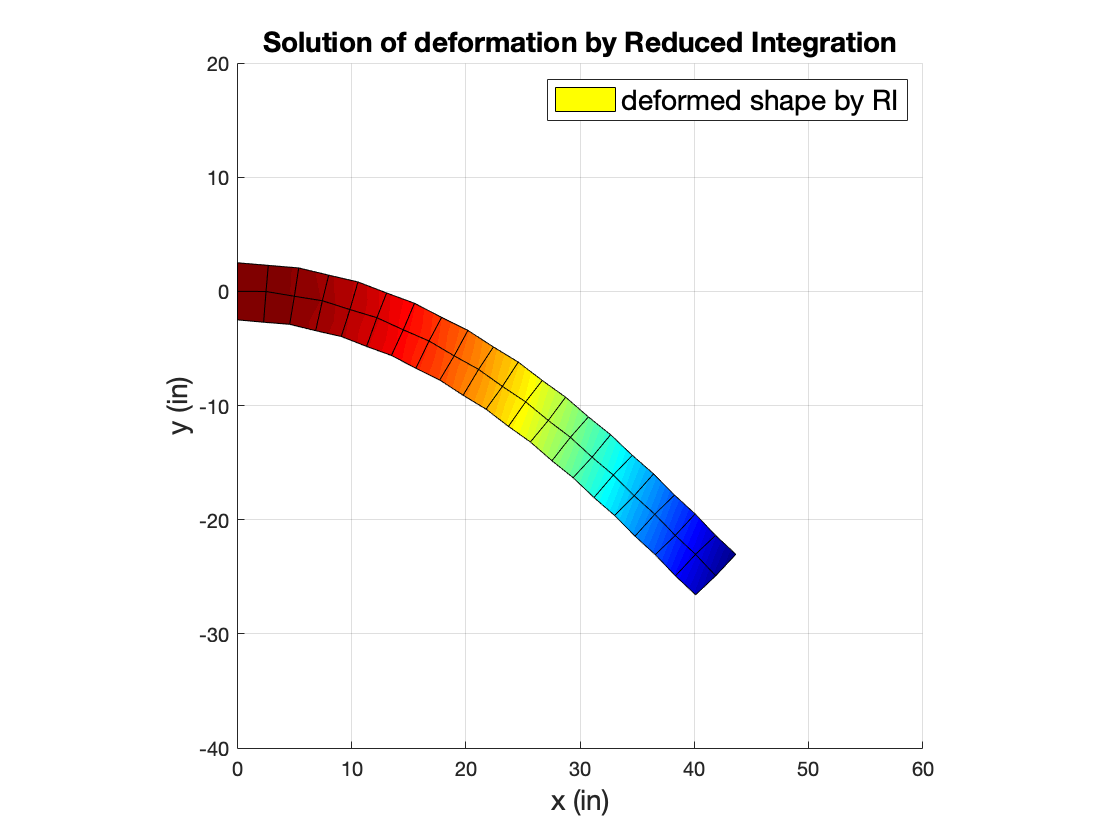
\includegraphics[width=7.1cm]{MAE232C_FINAL_PROJECT_latex/RI_1.png} }}
    \qquad
    \subfloat[Q4-SRI]{{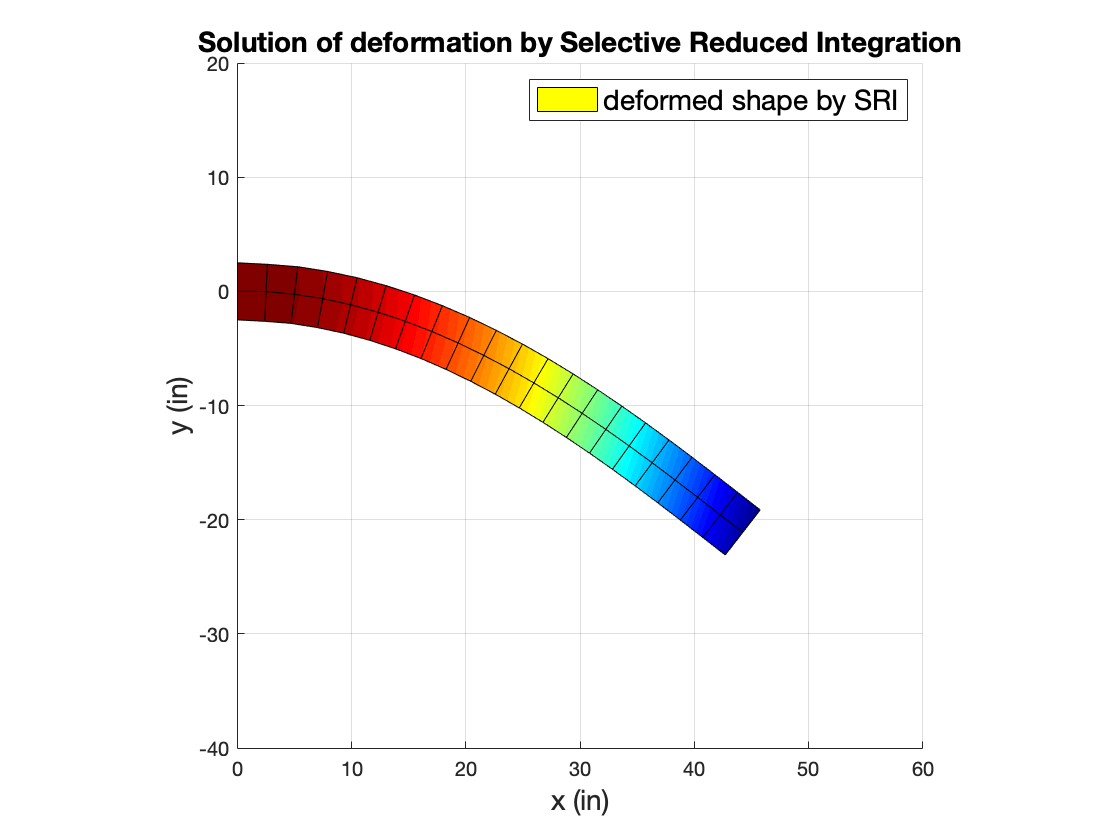
\includegraphics[width=7.1cm]{MAE232C_FINAL_PROJECT_latex/SRI_1.png} }}
    \qquad
    \subfloat[Q4-RI(enlarged)]{{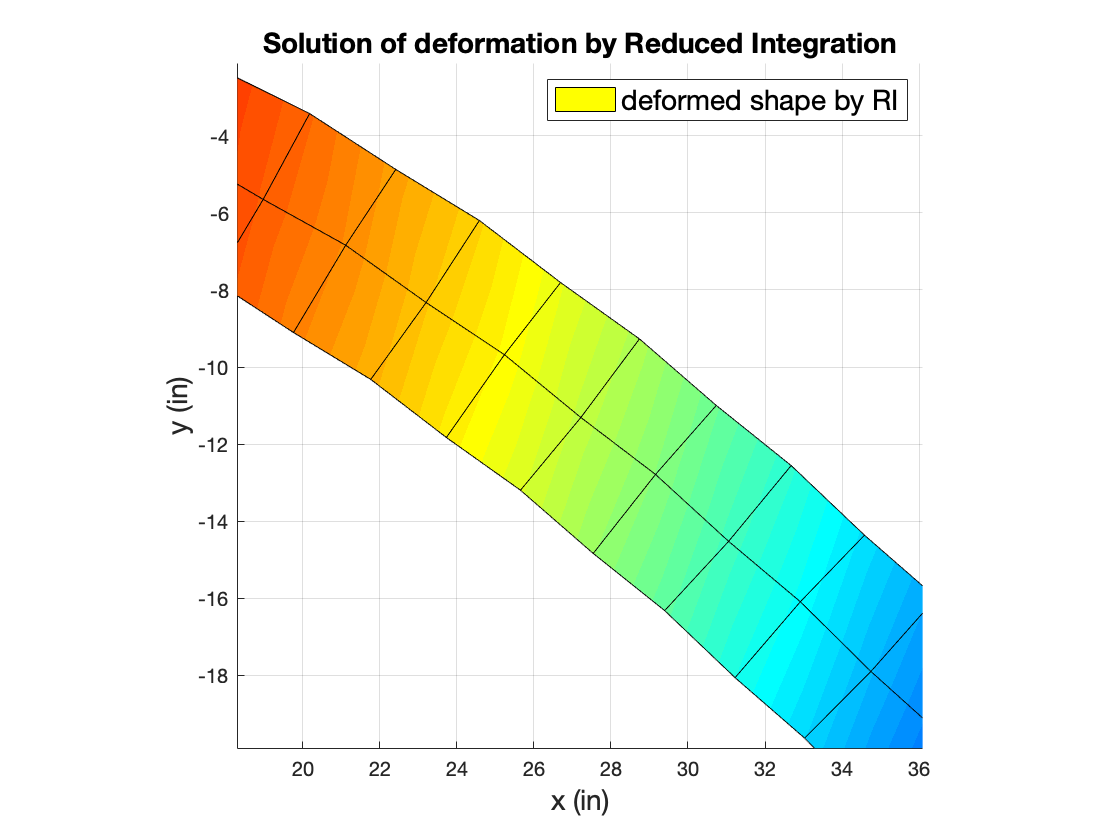
\includegraphics[width=7.1cm]{MAE232C_FINAL_PROJECT_latex/RI_1_L.png} }}
    \caption{Deformed shapes of beam when mesh = 2x20}
\end{figure}


\vspace*{1.5em}

\subsection{The Effect of Mesh Refinements on the Accuracy of Displacements and Stresses}

\vspace*{0.5em}
To study the effect of mesh refinement on accuracy, we can estimate the error of displacement by FI, RI and SRI, with 2x20, 4x40 and 8x80 meshing.
In Fig.7, the x axis is log(number of elements in x), representing mesh refinements. This means we have finer mesh when x is large. And the y axis is the absolute value of error for $u_y$ at the tip centroid when $P = 250 lb$. For all the three integration methods, error decreased as we refine the mesh. However, the error for FI does not converge to zero while the other two converge. 

Regarding the results of stresses, recalling Fig.4 and 5, we find the results of RI get closer to the results of SRI, which is set as the reference, as we refine the mesh. However, the results of FI could hardly be improved by mesh refinement.

Then we can conclude the locking effect in FI cannot be resolved by mesh refinement. But the results accuracy of RI and SRI (especially RI) can be greatly improved with finer mesh. And the results by SRI are more accurate than the results by RI because it uses more integration points to increase accuracy and also avoid hourglass instability.

\begin{figure}[H]
    \centering
    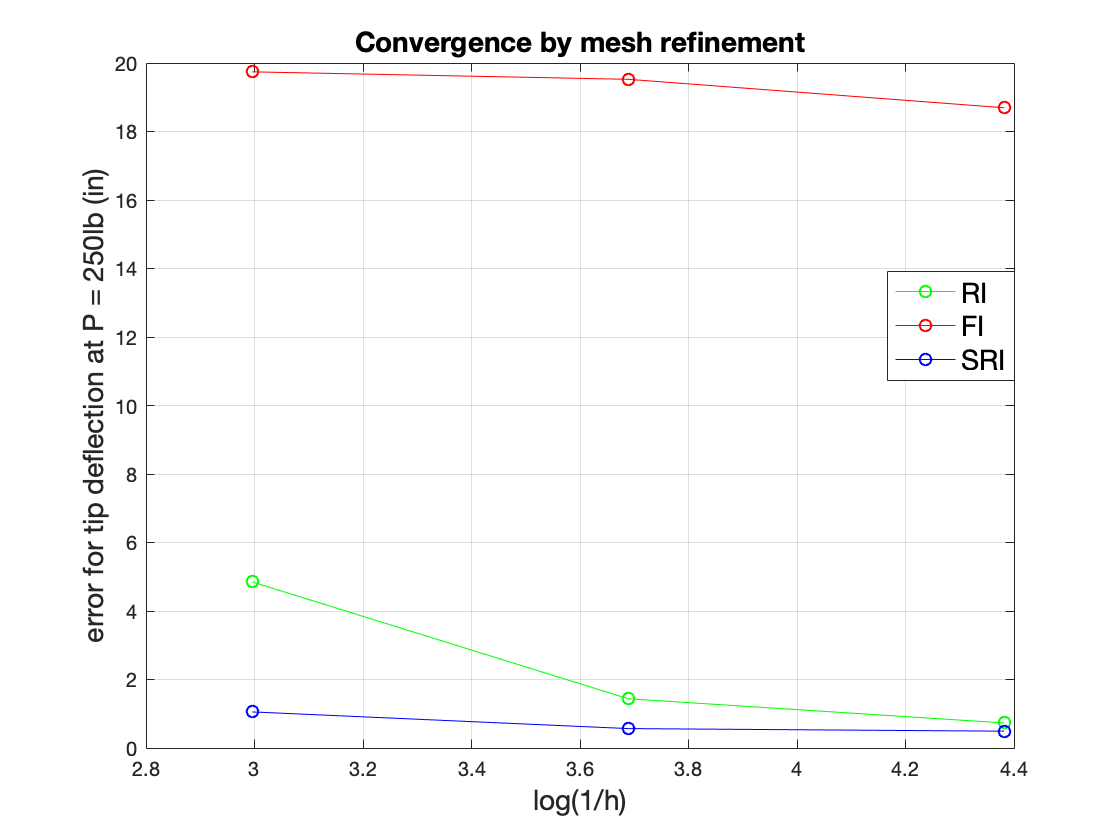
\includegraphics[width=11cm]{error.png}
    \caption{Error of $u_y$ at the tip centroid vs. mesh refinement}
\end{figure}

\vspace*{1.5em}



\end{document}